% !TEX program = lualatex
\documentclass[12pt,a4paper]{article}
\usepackage{graphicx}
\usepackage{fontspec}
\setmonofont{Latin Modern Mono}
\usepackage{xcolor}
\usepackage{listings}
\usepackage{geometry}
\usepackage{fancyhdr}
\usepackage{hyperref}
\usepackage{booktabs} 
\usepackage{float}    
\usepackage{amsmath}

% =======================================================
%  USER CONFIGURATION
% =======================================================
\newcommand{\labNo}{Lab 11}
\newcommand{\labTopic}{PL/pgSQL Named Blocks: Functions and Procedures}
\newcommand{\courseCode}{CSE 4308}
\newcommand{\courseTitleShort}{DBMS Lab}
\newcommand{\courseTitleLong}{DATABASE MANAGEMENT SYSTEMS LAB}
\newcommand{\instructorName}{Samnun Azfar, Jr. Lecturer, CSE\\ Samia Nawsheen, Jr. Lecturer, CSE}
\newcommand{\academicYear}{AY25-26}

% --- SOLUTION TOGGLE ---
% Change \showsolutionstrue to \showsolutionsfalse to generate 
% the student version (hidden answers).
\newif\ifshowsolutions
   \showsolutionstrue 
%\showsolutionsfalse
% =======================================================

\geometry{margin=1in}

% -
% Header and Footer Configuration
% -
\pagestyle{fancy}
\fancyhf{}
\lhead{\labNo}                        % Uses variable
\rhead{\courseCode: \courseTitleShort} % Uses variables

% Centered footer with page number
\cfoot{\thepage}
% Ensure header/footer width matches text block
\setlength{\headwidth}{\textwidth}

% -
% Code Listing Style
% -
\definecolor{codegreen}{rgb}{0,0.6,0}
\definecolor{codegray}{rgb}{0.5,0.5,0.5}
\definecolor{codepurple}{rgb}{0.58,0,0.82}
\definecolor{backcolour}{rgb}{0.95,0.95,0.92}

\lstdefinestyle{mystyle}{
    backgroundcolor=\color{backcolour},
    commentstyle=\color{codegreen},
    keywordstyle=\color{magenta},
    numberstyle=\tiny\color{codegray},
    stringstyle=\color{codepurple},
    basicstyle=\ttfamily\footnotesize,
    breaklines=true,
    captionpos=b,
    keepspaces=true,
    numbers=left,
    numbersep=5pt,
    tabsize=2,
    frame=single,
    numbers=none,
    columns=fullflexible,
    showspaces=false,
    showstringspaces=false,
    showtabs=false,
}

\lstset{style=mystyle}

% Images: found next to this file (local compile_labs.sh) or via the
% lab folder when compiled from the project root (Overleaf).
\graphicspath{{lab_11_function_procedure/}}

\begin{document}

% --
% TITLE PAGE
% --
\begin{titlepage}
    \centering
    \vspace*{2\baselineskip}

    \rule{14cm}{2pt}\vspace*{-0.8\baselineskip}\vspace*{1.5pt}
    \rule{14cm}{0.5pt}\vspace{2\baselineskip}

    {\Huge\bfseries\scshape \labNo\par} % Uses variable
    \vspace{3mm}
    {\Large \labTopic} % Uses variable
    \vspace{3mm}

    \rule{14cm}{0.5pt}\vspace*{-0.7\baselineskip}\vspace{2.5pt}
    \rule{14cm}{2pt}

    \vspace{2\baselineskip}

    {\Large\bfseries \courseCode\par} % Uses variable
    \vspace{1\baselineskip}
    {\large \courseTitleLong\par} % Uses variable

    \vfill
    {\normalsize Prepared by:\\ \instructorName\par} % Uses variable
    {\normalsize Academic Year: \academicYear\par} % Uses variable
\end{titlepage}

\newpage
\tableofcontents
\newpage

% =======================================================
% SECTION: LAB WORKFLOW
% =======================================================
\section{Lab Workflow}



\textit{Repeat this subsection for every single lab.}

\begin{enumerate}
\item Connect to the internet by running nmtui in terminal, add a dsl connection, then go back and activate that dsl connection. Make sure that your net id is not being used in any other pc or router, if you face any issue, use any other net id from your friends which is not being used.

\item Download all the files posted in the google classroom.

\item Disconnect from the \textbf{dsl} connection via nmtui, connect to the ethernet/wired connection via nmtui. If no such connection exists, create an \textbf{ethernet} connection  and then activate.

    \item \textbf{Create Your Role and Database}

Inside the PostgreSQL shell, create your own role (user) and database.

1. In the Linux terminal:
\begin{lstlisting}[language=bash]
psql
\end{lstlisting}

Expected prompt:
\begin{lstlisting}
cse=#
\end{lstlisting}

2. Create Your Role and Database

Copy and run the following commands inside PostgreSQL:
\begin{lstlisting}[language=SQL]
-- 1. Terminate existing database connections
SELECT pg_terminate_backend(pid)
FROM pg_stat_activity
WHERE datname = 'cse4308_12345'
  AND pid <> pg_backend_pid();

-- 2. Remove existing database
DROP DATABASE IF EXISTS cse4308_12345;

-- 3. Remove existing role
DROP ROLE IF EXISTS student_12345;

-- 4. Create role
CREATE ROLE student_12345 LOGIN;

-- 5. Set password
ALTER ROLE student_12345
WITH PASSWORD 'student12345';

-- 6. Create database
CREATE DATABASE cse4308_12345
OWNER student_12345;

-- 7. Grant privileges
GRANT ALL PRIVILEGES
ON DATABASE cse4308_12345
TO student_12345;
\end{lstlisting}

3. Exit PostgreSQL:

   \begin{lstlisting}[language=SQL]
   \q
   \end{lstlisting}

\item \textbf{Connect Using Your Newly Created User}

1. Connect to Your Database:

   Use the following command to log in as the \texttt{student\_12345} user:

   \begin{lstlisting}[language=SQL]
   psql -h localhost -U student_12345 -d cse4308_12345
   \end{lstlisting}

2. Verify the Connection:

   Verify that you are connected to the correct database with the following command:

   \begin{lstlisting}[language=SQL]
   \conninfo
   \end{lstlisting}

   Expected output:

   \begin{lstlisting}
   Database: cse4308_12345, User: student_12345
   \end{lstlisting}

3. Exit PostgreSQL:

   \begin{lstlisting}[language=SQL]
   \q
   \end{lstlisting}

\item \textbf{Load the Lab SQL File (MUST be run outside psql)}

Load the SQL file that sets up the tables and inserts initial data.

1. Load the SQL File:

   Run the following command to load the lab SQL file:

   \begin{lstlisting}[language=SQL]
   psql -h localhost -U student_12345 -d cse4308_12345 -f /home/cse/Downloads/lab_11_setup.sql
   \end{lstlisting}

   This will:
   - Drop old tables (if they exist).
   - Create new tables.
   - Insert initial rows of data.

\item \textbf{Reconnect and Verify Tables}

After loading the SQL file, reconnect to PostgreSQL to verify that the tables have been created.

1. Reconnect to Your Database:

   \begin{lstlisting}[language=SQL]
   psql -h localhost -U student_12345 -d cse4308_12345
   \end{lstlisting}

2. Check Tables:

   Verify the tables have been created by listing them:

   \begin{lstlisting}[language=SQL]
   \dt
   \end{lstlisting}

3. View Table Data:

   Verify the data by running the following SQL queries:

   \begin{lstlisting}[language=SQL]
   SELECT * FROM <table_name>;
   \end{lstlisting}

\item Open a text editor and save it in the appropriate submission name format \\ \texttt{fullid\_CSE4308\_L11\_T1.sql}. You will use this text editor to write your solutions, make sure to save it after writing each solution. The structure of this file will be:
\begin{lstlisting}[language=SQL]
-- Task 1
INSERT INTO students (student_id, name, major, gpa)
VALUES (104, 'David', 'ME', 3.60);
--Task 2
SELECT name, gpa FROM students WHERE major = 'CSE';
\end{lstlisting}
\end{enumerate}
% =======================================================
% SECTION: DATABASE SCHEMA
% =======================================================
\newpage
\section{Database Schema \& Data Generation}
\textbf{Instructions:} Save this code as \texttt{lab\_11\_setup.sql} and run it using \texttt{\textbackslash i lab\_11\_setup.sql} in your \texttt{psql} terminal. This script generates an e-commerce schema.

\begin{lstlisting}[language=SQL, caption={lab\_11\_setup.sql}]
-- 1. CLEANUP
DROP TABLE IF EXISTS order_items CASCADE;
DROP TABLE IF EXISTS orders CASCADE;
DROP TABLE IF EXISTS restock_logs CASCADE;
DROP TABLE IF EXISTS products CASCADE;
DROP TABLE IF EXISTS customers CASCADE;

-- 2. CREATE TABLES
CREATE TABLE customers (
    customer_id SERIAL PRIMARY KEY,
    name VARCHAR(100),
    region VARCHAR(50),
    loyalty_tier VARCHAR(20) -- 'Bronze', 'Silver', 'Gold', 'Platinum'
);

CREATE TABLE products (
    product_id SERIAL PRIMARY KEY,
    name VARCHAR(100),
    category VARCHAR(50),
    base_price NUMERIC(10, 2),
    stock_quantity INT
);

CREATE TABLE orders (
    order_id SERIAL PRIMARY KEY,
    customer_id INT REFERENCES customers(customer_id),
    order_date DATE,
    status VARCHAR(20), -- 'PENDING', 'PROCESSED', 'PARTIAL', 'CANCELLED'
    total_value NUMERIC(12, 2) DEFAULT 0.00
);

CREATE TABLE order_items (
    item_id SERIAL PRIMARY KEY,
    order_id INT REFERENCES orders(order_id) ON DELETE CASCADE,
    product_id INT REFERENCES products(product_id),
    quantity INT,
    unit_price NUMERIC(10, 2)
);

CREATE TABLE restock_logs (
    log_id SERIAL PRIMARY KEY,
    product_id INT REFERENCES products(product_id),
    restock_date DATE,
    added_quantity INT
);

-- 3. DATA GENERATION
-- Insert 1000 Customers
INSERT INTO customers (name, region, loyalty_tier)
SELECT 
    'Customer_' || id,
    (ARRAY['North', 'South', 'East', 'West'])[floor(random() * 4 + 1)],
    (ARRAY['Bronze', 'Silver', 'Gold', 'Platinum'])[floor(random() * 4 + 1)]
FROM generate_series(1, 1000) AS id;

-- Insert 200 Products
INSERT INTO products (name, category, base_price, stock_quantity)
SELECT 
    'Product_' || id,
    (ARRAY['Electronics', 'Clothing', 'Groceries', 'Tools', 'Books'])[floor(random() * 5 + 1)],
    ROUND((random() * 500 + 10)::numeric, 2),
    floor(random() * 100 + 10)::INT
FROM generate_series(1, 200) AS id;

-- Insert 3000 Orders (Statuses randomized)
INSERT INTO orders (customer_id, order_date, status)
SELECT 
    floor(random() * 1000 + 1)::INT,
    CURRENT_DATE - (floor(random() * 365)::INT),
    (ARRAY['PENDING', 'PROCESSED', 'PROCESSED', 'PARTIAL', 'CANCELLED'])[floor(random() * 5 + 1)]
FROM generate_series(1, 3000);

-- Insert 9000 Order Items (Averaging 3 items per order)
INSERT INTO order_items (order_id, product_id, quantity, unit_price)
SELECT 
    floor(random() * 3000 + 1)::INT,
    floor(random() * 200 + 1)::INT,
    floor(random() * 5 + 1)::INT,
    0.00
FROM generate_series(1, 9000) ON CONFLICT DO NOTHING;

-- Fix the unit_price in order_items based on products table
UPDATE order_items oi
SET unit_price = p.base_price
FROM products p
WHERE oi.product_id = p.product_id;

-- Initial aggregation to set order total_values
UPDATE orders o
SET total_value = sub.total
FROM (
    SELECT order_id, COALESCE(SUM(quantity * unit_price), 0) as total 
    FROM order_items 
    GROUP BY order_id
) sub
WHERE o.order_id = sub.order_id;
\end{lstlisting}

\begin{figure}[h]
    \centering
    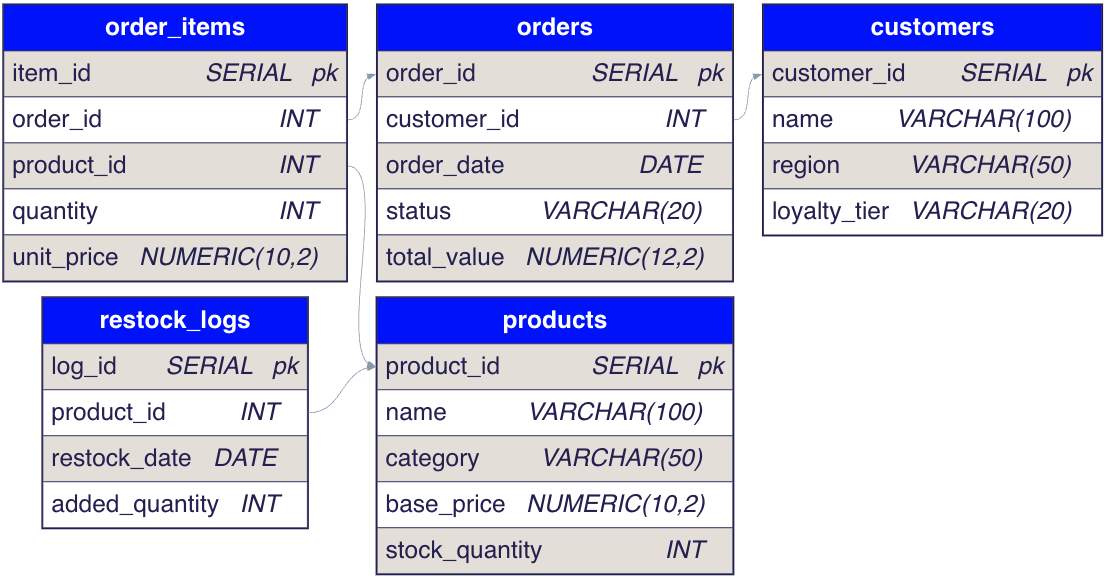
\includegraphics[width=0.7\linewidth]{lab_11_figure.png}
\end{figure}
% =======================================================
% SECTION: INTRODUCTION TO NAMED BLOCKS
% =======================================================
\newpage
\section{Introduction to Named Blocks}
Anonymous blocks (\texttt{DO \$\$}) evaluate procedural logic for single execution but are not persistently stored in the database schema. Persistent named blocks, referred to as subprograms, encapsulate procedural logic for reuse. In PostgreSQL, subprograms are classified into two primary constructs: \textbf{User-Defined Functions} and \textbf{Stored Procedures}.

\subsection{User-Defined Functions}
A named PL/pgSQL block that evaluates to a specific return type. Functions are invoked within expressions (e.g., a \texttt{SELECT} statement) and structurally require a \texttt{RETURN} or \texttt{RETURN QUERY} statement. They execute entirely within the transaction scope of the invoking query; they cannot execute Transaction Control Language (TCL) commands such as \texttt{COMMIT} or \texttt{ROLLBACK}.

\subsection{Stored Procedures}
A named PL/pgSQL block invoked via the \texttt{CALL} statement. Procedures do not evaluate to a direct return value and are capable of autonomous transaction control. This capability dictates their use for bulk data manipulation, schema migrations, and batch processing workflows.

% =======================================================
% SECTION: PARAMETER MODES
% =======================================================
\section{Parameter Modes}
Formal parameters in PL/pgSQL are assigned a mode that dictates the direction of data binding between the calling environment and the subprogram.

\begin{itemize}
    \item \textbf{\texttt{IN} Mode (Implicit Default):} Specifies that the formal parameter accepts an actual argument from the caller. It is lexically immutable (read-only) within the subprogram body.
    \item \textbf{\texttt{OUT} Mode:} Specifies an uninitialized variable bound to the caller's environment. The subprogram assigns a value to it, which is transmitted back upon termination.
    \item \textbf{\texttt{INOUT} Mode:} A hybrid parameter that accepts an initialized actual argument from the caller, permits state mutation within the subprogram body, and transmits the modified state back to the caller upon termination.
\end{itemize}

% =======================================================
% SECTION: DEFINING SUBPROGRAMS
% =======================================================
\section{Defining the Subprograms}
Before invoking them dynamically, subprograms must be compiled into the schema.

\begin{lstlisting}[language=SQL, caption={Scalar Function Example}]
CREATE OR REPLACE FUNCTION calculate_customer_lifetime_value(p_cust_id INT)
RETURNS NUMERIC AS $$
DECLARE
    v_total_spent NUMERIC;
BEGIN
    SELECT COALESCE(SUM(total_value), 0) INTO v_total_spent
    FROM orders
    WHERE customer_id = p_cust_id;
    
    RETURN v_total_spent;
END;
$$ LANGUAGE plpgsql;
\end{lstlisting}

\begin{lstlisting}[language=SQL, caption={Procedure Example with Mixed Modes and TCL}]
CREATE OR REPLACE PROCEDURE process_category_discount(
    p_category IN VARCHAR,      -- Read-only constraint
    p_discount_budget INOUT NUMERIC,   -- Mutated and returned to caller
    p_budget_status OUT VARCHAR -- Assigned and returned to caller
)
LANGUAGE plpgsql AS $$
DECLARE
    v_product_count INT;
BEGIN
    -- Utilize IN parameter for scalar subquery
    SELECT COUNT(*) INTO v_product_count
    FROM products
    WHERE category = p_category;
    
    -- Transform the INOUT parameter
    p_discount_budget := p_discount_budget - (v_product_count * 50.00);
    
    -- Initialize the OUT parameter
    IF p_discount_budget > 0 THEN
        p_budget_status := 'BUDGET_SURPLUS';
    ELSE
        p_budget_status := 'BUDGET_DEFICIT';
    END IF;
    
    -- Procedural Transaction Control
    COMMIT;
END;
$$;
\end{lstlisting}

% =======================================================
% SECTION: EXECUTION INSIDE ANONYMOUS BLOCKS
% =======================================================
\section{Execution Inside Anonymous Blocks}
This is the standard methodology for testing or dynamically invoking procedural logic without saving a new script to the database schema. Because anonymous blocks cannot return result sets directly to the client interface like a standard \texttt{SELECT} statement, you must utilize the \texttt{DECLARE} section to capture outputs and \texttt{RAISE NOTICE} to observe the results.

\subsection{Calling a Function}
Functions evaluate to a value. Inside a block, you must either assign this evaluated value to a declared variable using the \texttt{:=} operator, or use \texttt{SELECT ... INTO}.

\begin{lstlisting}[language=SQL, caption={Calling a Function}]
DO $$
DECLARE
    -- 1. Declare a variable to hold the function's return payload
    v_ltv NUMERIC;
BEGIN
    -- 2. Assign the function evaluation directly to the variable
    v_ltv := calculate_customer_lifetime_value(1);
    
    -- 3. Output the state
    RAISE NOTICE 'Customer LTV: %', v_ltv;
END;
$$;
\end{lstlisting}

\subsection{Calling a Procedure}
Procedures are invoked using the \texttt{CALL} statement. When a procedure utilizes \texttt{OUT} or \texttt{INOUT} parameters, you cannot pass raw literals into those parameter slots. You must pass \textbf{variables by reference} so the procedure has a memory address to write the modified state back to.

\begin{lstlisting}[language=SQL, caption={Calling a Procedure}]
DO $$
DECLARE
    -- 1. Initialize variables for INOUT parameters
    v_promo_budget NUMERIC := 10000.00; 
    
    -- 2. Declare uninitialized variables for OUT parameters
    v_status VARCHAR;  
BEGIN
    -- 3. Execute the procedure, passing the variables by reference
    CALL process_category_discount(
        'Electronics',   -- IN argument (literal is fine here)
        v_promo_budget,  -- INOUT argument (must be a variable)
        v_status         -- OUT argument (must be a variable)
    );
    
    -- 4. The variables in this block's scope now hold the mutated states
    RAISE NOTICE 'Remaining Budget: %, Status: %', v_promo_budget, v_status;
END;
$$;
\end{lstlisting}

% =======================================================
% SECTION: LAB TASKS
% =======================================================
\newpage
\section{Lab Tasks}
\begin{enumerate}

% Task 1
    \item Create a function named \texttt{get\_cross\_sell\_recommendations} that accepts a \\\texttt{p\_target\_product\_id} parameter. The function will:
    \begin{itemize}
        \item Find all orders that contain this target product.
        \item Identify what \textit{other} products were bought in those same orders.
        \item Return a table containing the top 3 most frequently co-purchased products.
        \item The output table should have columns: \texttt{rec\_product\_id}, \texttt{rec\_name}, and \texttt{co\_buy\_count}.
    \end{itemize}

    \ifshowsolutions
    \textbf{Solution:}
    \begin{lstlisting}[language=SQL]
CREATE OR REPLACE FUNCTION get_cross_sell_recommendations(p_target_product_id INT)
RETURNS TABLE (rec_product_id INT, rec_name VARCHAR, co_buy_count INT) 
LANGUAGE plpgsql AS $$
BEGIN
    RETURN QUERY
    SELECT oi.product_id, p.name, COUNT(*)::INT as frequency
    FROM order_items oi JOIN products p USING (product_id)
    WHERE oi.order_id IN (SELECT order_id FROM order_items WHERE product_id = p_target_product_id)
      AND oi.product_id != p_target_product_id
    GROUP BY oi.product_id, p.name ORDER BY frequency DESC LIMIT 3;
END; 
$$;

DO $$
DECLARE
    -- Record variable to hold each row returned by the function
    v_rec RECORD;
    v_target_product_id INT := 1; -- We are checking recommendations for Product_1
BEGIN
    RAISE NOTICE 'Finding Cross-Sell Recommendations for Product ID %...', v_target_product_id;

    -- Iterate through the table returned by the function
    FOR v_rec IN SELECT * FROM get_cross_sell_recommendations(v_target_product_id) 
    LOOP
        RAISE NOTICE 'Recommendation: Product ID %, Name: %, Co-Buy Frequency: %', 
                     v_rec.rec_product_id, 
                     v_rec.rec_name, 
                     v_rec.co_buy_count;
    END LOOP;
    
    -- If no results found (loop didn't run), you might see nothing. 
    -- This ensures we know the block finished.
    RAISE NOTICE '-------------------------------------------';
    RAISE NOTICE 'Analysis Complete.';
END;
$$;
    \end{lstlisting}
    \fi

% Task 2
    \item Create a procedure named \texttt{auto\_restock\_depleted} that takes three parameters: \texttt{p\_threshold} (IN), \texttt{p\_restock\_amount} (IN), and \texttt{p\_total\_cost} (OUT).
    \begin{itemize}
        \item Identify all products where the stock quantity is less than the threshold.
        \item For each low-stock product, increase the stock by the restock amount.
        \item Insert a record into the \texttt{restock\_logs} table.
        \item Calculate the cost (assume wholesale cost is 40\% of base price) and add it to the total cost.
    \end{itemize}

    \ifshowsolutions
    \textbf{Solution:}
    \begin{lstlisting}[language=SQL]
CREATE OR REPLACE PROCEDURE auto_restock_depleted(IN p_threshold INT, IN p_restock_amount INT, OUT p_total_cost NUMERIC) 
LANGUAGE plpgsql AS $$
DECLARE
    v_prod RECORD;
BEGIN
    p_total_cost := 0.00;

    FOR v_prod IN SELECT product_id, base_price FROM products WHERE stock_quantity < p_threshold LOOP
        UPDATE products SET stock_quantity = stock_quantity + p_restock_amount WHERE product_id = v_prod.product_id;
        INSERT INTO restock_logs (product_id, restock_date, added_quantity) VALUES (v_prod.product_id, CURRENT_DATE, p_restock_amount);
        p_total_cost := p_total_cost + ((v_prod.base_price * 0.40) * p_restock_amount);
    END LOOP;
    COMMIT;
END; 
$$;

DO $$
DECLARE
    -- 1. Declare variable to hold the OUT parameter (Total Cost)
    v_total_cost NUMERIC;
    
    -- Variable for verification count
    v_restocked_count INT;
BEGIN
    -- 2. Call the procedure
    -- Arguments: 
    --   p_threshold = 20 (Restock items with < 20 stock)
    --   p_restock_amount = 50 (Add 50 units to those items)
    --   p_total_cost = v_total_cost (Capture the output variable)
    CALL auto_restock_depleted(20, 50, v_total_cost);

    -- 3. Output the result from the procedure
    RAISE NOTICE 'Procedure execution complete.';
    RAISE NOTICE 'Total Cost of Restocking: $%', v_total_cost;

    -- 4. Verification: Check how many logs were inserted for today
    SELECT COUNT(*) INTO v_restocked_count 
    FROM restock_logs 
    WHERE restock_date = CURRENT_DATE;

    RAISE NOTICE 'Verification: % products were restocked today.', v_restocked_count;
END;
$$;
    \end{lstlisting}
    \fi

% Task 3
    \item
    Create a procedure named \texttt{anonymize\_inactive\_customers} that returns a count of modified rows via an OUT parameter (\texttt{p\_anonymized\_count}).
    \begin{itemize}
        \item A customer is considered "Inactive" if they have never placed an order OR their last order was more than 730 days ago.
        \item For every inactive customer, update their details to: Name = \texttt{'ANONYMIZED'}, Region = \texttt{'UNKNOWN'}, and Loyalty Tier = \texttt{'Bronze'}.
        \item Return the total number of customers who were anonymized.
    \end{itemize}

\ifshowsolutions
\textbf{Solution:}
\begin{lstlisting}[language=SQL]
CREATE OR REPLACE PROCEDURE anonymize_inactive_customers(OUT p_anonymized_count INT) 
LANGUAGE plpgsql AS $$
DECLARE
    v_cust RECORD;
BEGIN
    p_anonymized_count := 0;

    FOR v_cust IN 
        SELECT c.customer_id, COALESCE(CURRENT_DATE - MAX(o.order_date), 9999) AS days_inactive
        FROM customers c LEFT JOIN orders o USING (customer_id) GROUP BY c.customer_id
    LOOP
        IF v_cust.days_inactive > 730 THEN
            UPDATE customers SET name = 'ANONYMIZED', region = 'UNKNOWN', loyalty_tier = 'Bronze'
            WHERE customer_id = v_cust.customer_id;
            p_anonymized_count := p_anonymized_count + 1;
        END IF;
    END LOOP;
    COMMIT;
END; 
$$;


DO $$
DECLARE
    v_reported_count INT;
    v_actual_db_count INT;
BEGIN
    -- 1. Execute the procedure and capture the OUT parameter
    CALL anonymize_inactive_customers(v_reported_count);
    
    -- 2. Output the result reported by the procedure
    RAISE NOTICE 'Procedure Execution Complete.';
    RAISE NOTICE 'Reported Count: % customers anonymized.', v_reported_count;
    
    -- 3. Independent Verification Query
    -- Count how many rows actually possess the anonymized attributes in the table
    SELECT COUNT(*) INTO v_actual_db_count
    FROM customers
    WHERE name = 'ANONYMIZED' 
      AND region = 'UNKNOWN' 
      AND loyalty_tier = 'Bronze';
      
    -- 4. Evaluate the results
    RAISE NOTICE 'Database Verification Count: % rows found.', v_actual_db_count;
    
    IF v_reported_count = v_actual_db_count THEN
        RAISE NOTICE 'VERIFICATION SUCCESS: The procedure''s internal counter matches the physical database state.';
    ELSE
        RAISE NOTICE 'VERIFICATION FAILED: Data mismatch detected.';
    END IF;
END;
$$;
\end{lstlisting}
\fi
\end{enumerate}

\end{document}